Im Rahmen dieser Arbeit wurden zwei Systeme zur Erkennung von Hindernissen in Echtzeit entwickelt. Diese richten sich nach den in Kapitel REF erläuterten Algorithmen und Konzepten. Anhand dieser ist es möglich aus den beiden Bildern des Stereo Systems für jeden Frame die Disparity Map zu berechnen, welche im Anschluss daran in mehreren Schritten zunächst so angepasst wird, dass nicht verwertbare Bereiche der Tiefenkarte entfernt werden (siehe \ref{sec:bildaufnahme_preprocessing}). Dies reduziert die Anzahl der zur Erkennung zu verarbeitenden Punkte und somit die Rechenzeit.\\

\noindent
Im folgenden Kapitel werden beide Methoden detailliert beleuchtet. Zu Beginn wird die zugrunde liegende Klassenstruktur beschrieben. In Abschnitt \ref{sec:mean_disparity_detection} die \emph{Mean Disparity Detection} erläutert, wobei auf das grundlegende Konzept sowie den Algorithmus zur Erkennung selber eingegangen wird. Selbiges gilt für die \emph{Samplepoint Detection} in Abschnitt \ref{sec:samplepoint_detection}.


%\begin{figure}[h]
%	\begin{center}
%	    %TODO: change Samplepoint Detection mImageCenter to private
%	    %TODO: add Subimage Stuff to MeanDisparityDetection
%		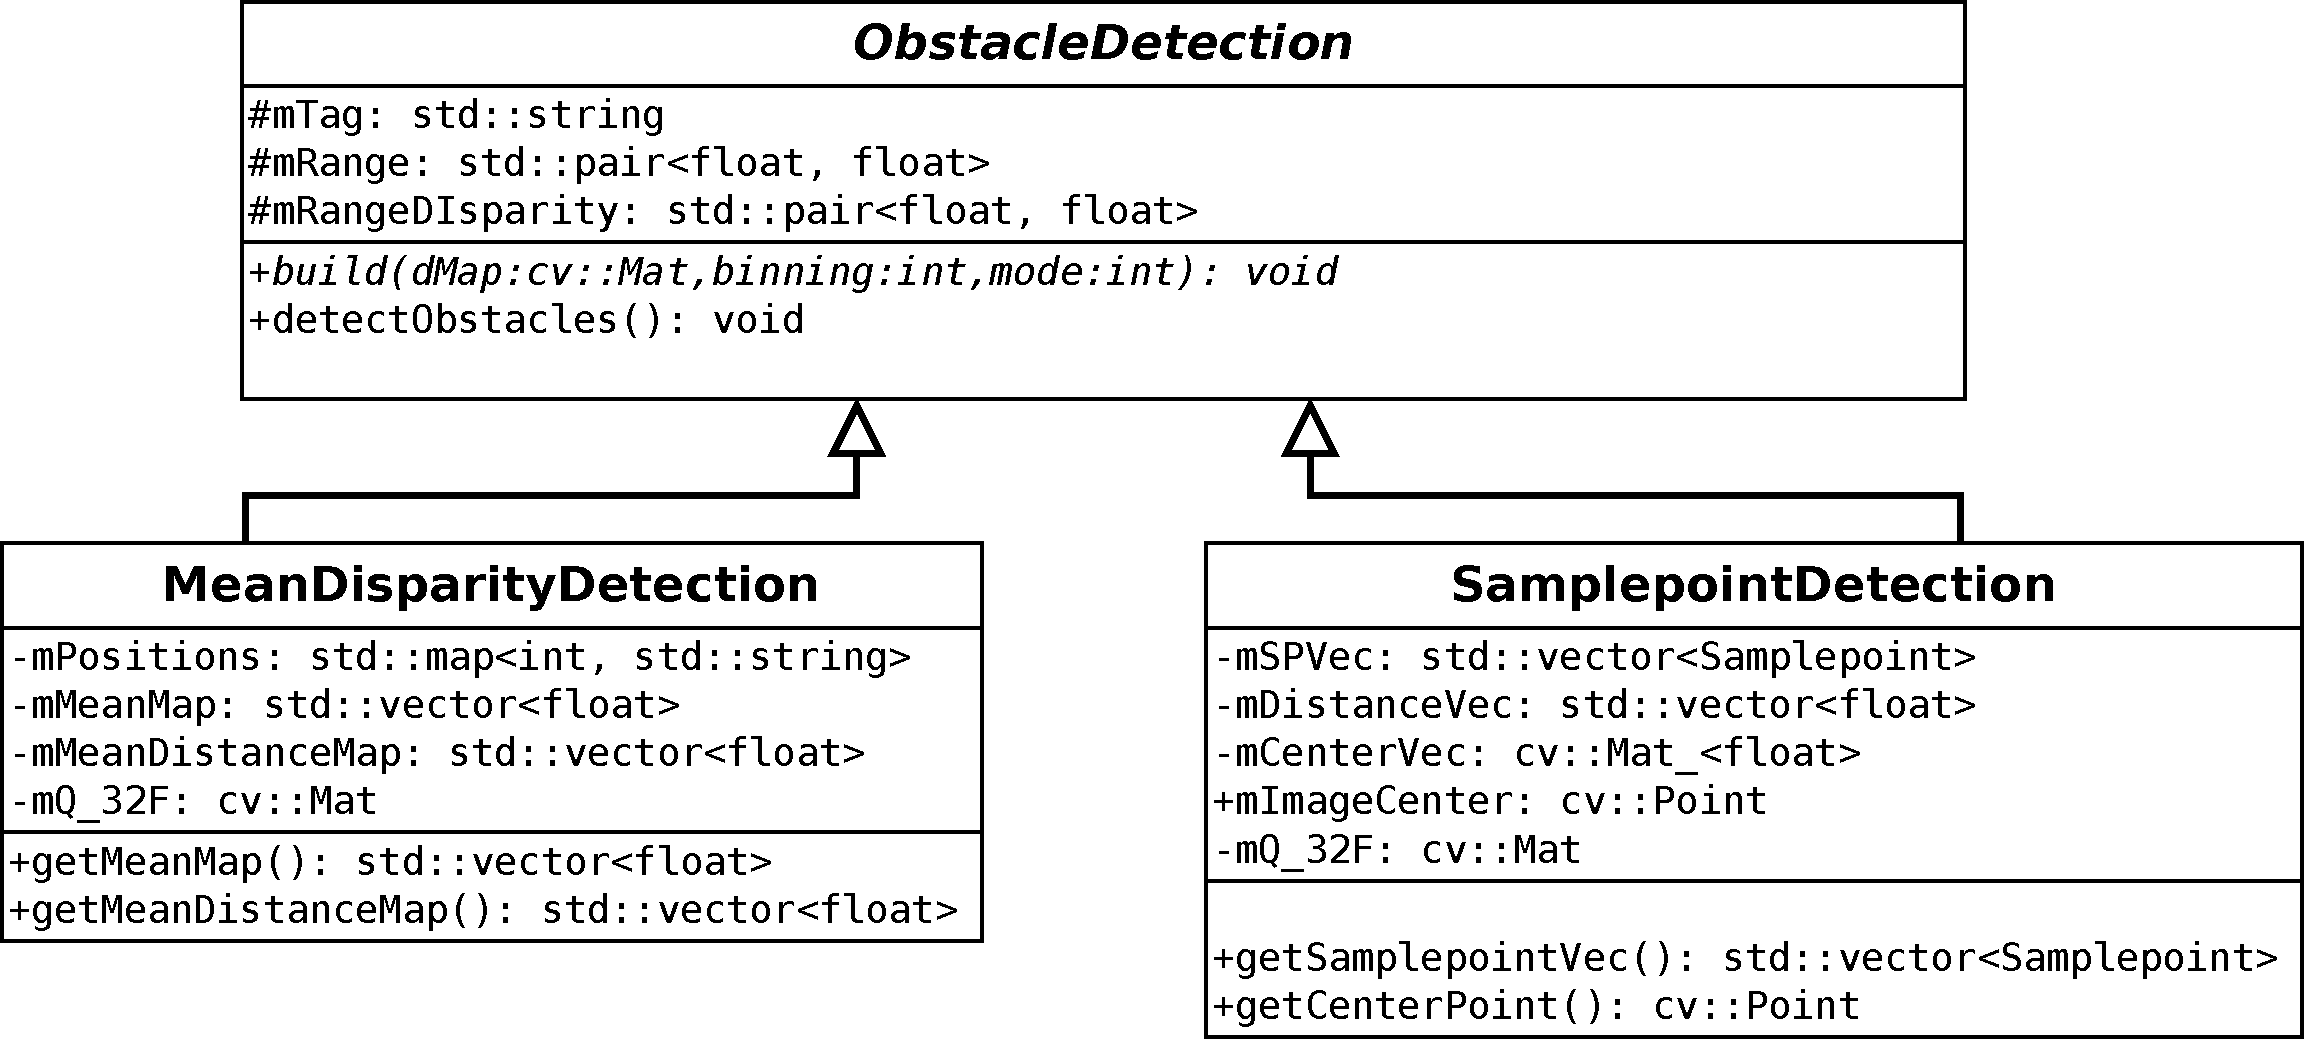
\includegraphics[width=13cm]{img/obstacle_detection_structure.pdf}
%	\end{center}
%	\caption{Klassenstruktur der Hinderniserkennung}
%	\label{fig:obstacle_detection_structure}
%\end{figure}



% ---------------------- section -----------------------
\section{Mean Disparity Detection}
\label{sec:mean_disparity_detection}

Das grundlegende Funktionsprinzip der \emph{Mean Disparity Detection} ist grob an die von Kostavelis et al. vorgestellten Algorithmen angelehnt. Auch bei diesen werden die berechneten Disparity Maps in Segmente eingeteilt von welchen in jedem Frame der Mittelwert errechnet wird.\\

\noindent
Zu Beginn des Algorithmus, nach der vorherigen Bearbeitung der eigentlichen \emph{region of interest}, wird während der Initialisierung die Segmentierung der Disparity Map festgelegt. Dabei wird für jedes Segment ein eigenes Subimage erzeugt. Diese definieren eine \emph{region of interest} (ROI) innerhalb einer Matrix. Subimages selber halten lediglich die Positionsinformationen (obere linke und untere rechte Ecke des definierten Rechtecks), Mittelwert der ROI, die ROI selbst sowie den Mittelpunkt des Rechtecks zur späteren Pointcloud Generierung, wie Abbildung \ref{fig:subimage_class} aufzeigt.

\begin{figure}[h]
	\begin{center}
		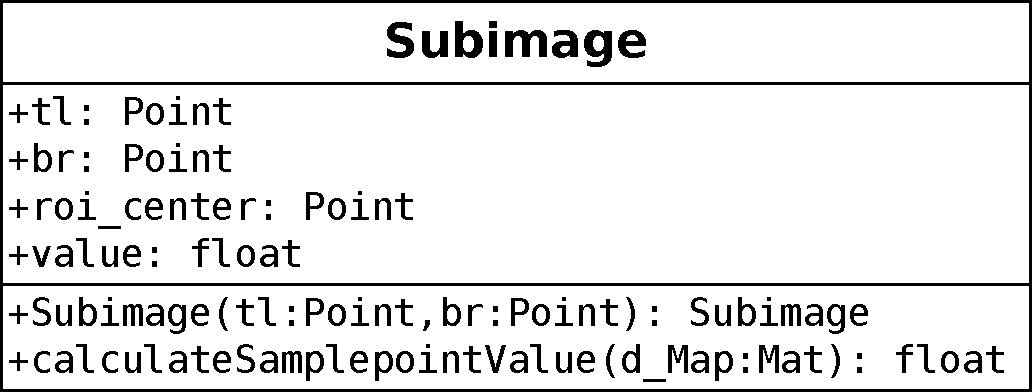
\includegraphics[width=8cm]{img/subimage_class.pdf}
	\end{center}
	\caption{Subimage Klasse}
	\label{fig:subimage_class}
\end{figure}

\noindent
Für die Unterteilung der Disparity Map wurden intial nur 9 Segmente vorgesehen wobei jeder Bereich eine der möglichen Flugrichtungen repräsentieren sollte. Aufgrund der Größe der Submatrizen konnte jedoch keine valide Erkennung kleiner Hindernisse gewährleistet werden, da solche in der Berechnung des Mittelwertes untergegangen sind. Aufgrund dessen wurde die Anzahl der Segmente auf 81 erhöht, welches eine wesentlich genauere Erkennung ermöglicht. Zudem ist somit eine weitaus genauere Einteilung der Flugrichtungen möglich, da jede dieser nocheinmal genauer betrachtet wird (siehe Abbildung \ref{fig:subimage_detection_segments}).

\begin{figure}[h]
	\begin{center}
		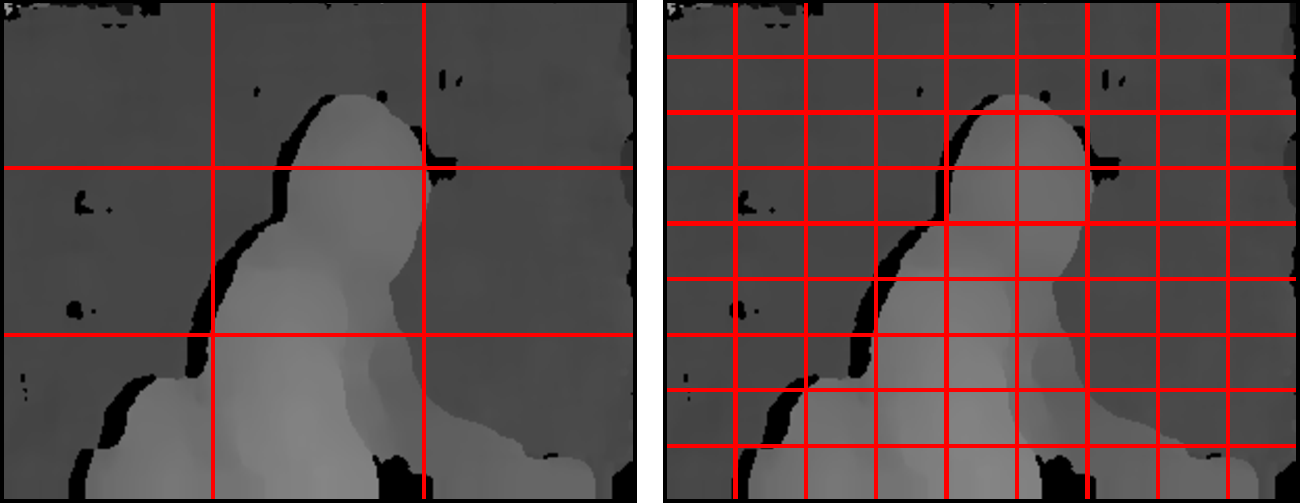
\includegraphics[width=10cm]{img/subimage_segmentation.pdf}
	\end{center}
	\caption{Intiale Segmentierung der Disparity Map sowie die weitere Unterteilung zur genaueren Bestimmung der Werte der Subimages}
	\label{fig:subimage_detection_segments}
\end{figure}

\noindent
Um die Hindernisse innerhalb der Segmente zu Erkennen wurde auf die Berechnung des Mittelwertes dieser gesetzt. Einerseits, da die Berechnung des Mittelwertes unter Betrachtung des Echtzeit-Aspektes eine ressourcensparende und schnelle Operation ist, andererseits weil jeder Pixel des Bildes in das Endresultat mit einfließt. Jedoch musste die Berechnung auf das Szenario angepasst werden, da Berechnung des Medians aller Werte zu Verzerrungen geführt hätte. Bei der Kalkulation von Disparity Maps werden Bereiche welche nicht gematcht werden können, sei es aufgrund von fehlenden Informationen im Referenzbild oder homogener Texturen in der Szene, als negativer Wert ausgedrückt. Berechnet man nun den Mittelwert unter Betrachtung positiver und negativer Werte, so entspricht dies zwar dem definierten Term Median, verfälscht allerdings das in diesem Anwendungsbereich erwünschte Ergebnis. Im schlechtesten Fall enthält eine Submatrix mehr negative als positive Werte, was dazu führen kann das Hindernisse vor homogenen Flächen nicht erkannt werden. Daraus ergibt sich die in Algorithmus \ref{alg:mean_disparity_calculation} dargestellte Berechnung des Mittelwertes.

\begin{algorithm}[h]
\caption{Berechnung des Disparity Medians}
\label{alg:mean_disparity_calculation}
\begin{algorithmic}[1]
    \Procedure{CalcMeanDisparity}{$submatrix$}
        \State $elements_{number} \gets 0$
        \State $elements_{sum} \gets 0 $
        \For{$value$ in $submatrix$}
            \If{$value > 0$}
                \State $elements_{sum} \gets elements_{sum} + value$
                \State $elements_{number} \gets elements_{number} + 1$
            \EndIf
        \EndFor
        \State \textbf{return} $elements_{sum} / elements_{number}$
    \EndProcedure
\end{algorithmic}  
\end{algorithm}

\noindent
Es werden demnach nur positive Disparitäten betrachtet was auch dazu führt das sich der Gesamtwert aller Werte aus der Menge dieser ergibt. Mit Hilfe dieser Berechnung ist es möglich Hindernisse auch in Bereichen zu erkennen in denen die Mehrzahl der Pixel keine Matches aufweisen.\\

\noindent
Die eigentliche Hinderniserkennung erfolgt in jedem Frame. Wobei der Term Frame hierbei nicht nach einem von der Kamera aufgenommenen Bild, sondern eine neue Disparity Map definiert. Da die Bildgröße pro Einzelbild stetig ist besteht keine Nötigkeit die einzelnen Segmente erneut zu generieren. Es genügt also die Mittelwerte eines jeden Subimages anhand der neuen Disparity Map zu aktualisieren. Daraufhin wird geprüft ob sich einer oder mehrere der Subimage Mittelwerte innerhalb der Gefahrenzone befinden. Die Gefahrenzone wird zur Initialisierung der Erkennung berechnet. Da die Disparitäten in Abhängigkeit der Bildgröße sowie der Q-Matrix berechnet werden ergibt kann kein fest definierter Disparitätenwert für eine Distanz bestimmt werden. Demnach müssen zu Beginn die minimale sowie maximale Distanz der Erkennung auf einen Tiefenwert zurückgerechnet werden (siehe Formel \ref{eq:backward_calculation}). Dies erfolgt als Erweiterung der in Abschnitt \ref{sec:framework} beschriebenen ursprünglichen Distanzberechnung.\\

\begin{equation}
  \label{eq:backward_calculation}
  \begin{aligned}
    d &= \frac{f- Z' \cdot b}{Z' \cdot a}\\
    I_x &= X' \cdot (d \cdot a + b) + C_x\\
    I_y &= Y' \cdot (d \cdot a + b) + C_y
  \end{aligned}
\end{equation}

\noindent
Diese Rückrechnung ist ausschlaggebend für die schnelle Erkennung der Tiefe. Im Falle einer weiteren Segmentierung müsste die Berechnung der Distanz für jedes Subimage einzeln erfolgen, was gerade bei der Samplepoint Detecion zum Tragen kommt, sollen die Distanzen für ca. $6000$ Punkte (bei voller Auflösung in Abhängigkeit der verwendeten Parameter des SGBM) berechnet werden.\\

% TODO subimage detection pseudocode
\begin{algorithm}[h]
\caption{Ablauf der Hinderniserkennung}
\label{alg:mean_disparity_detection}
\begin{algorithmic}[1]
    \Procedure{detectObstacles}{$submatrix$}
		\State $found\_points \gets 0$
		\State $found\_obstacles \gets 0$
		\For{$value$ in $mean\_disparities$}
			\If{$value < range_{min}$ AND $value > range_{max}$}
				\State $temp\_Subimage \gets Subimage\_vector[index_{value}]$
				\State $found\_obstacles \gets found\_obstacles.append(value)$
				\State $coordinate \gets calc\_coordinate(temp\_Subimage$
    \EndProcedure
\end{algorithmic}  
\end{algorithm}

\noindent
Die in Algorithmus \ref{alg:mean_disparity_detection} berechnete Pointcloud ist in diesem Fall ein Matrix mit der Größe der ursprünglichen Tiefenkarte. Dies ist für die Berechnung der dreidimensionalen Koordinate von Nöten. Mithilfe des Mittelpunkte der Subimages wird für jedes dieser die jeweilige 3D-Koordinate (siehe Abschnitt \ref{sec:framework}) berechnet und an der Position des Mittelwertes in die Punktwolke geschrieben.

\noindent
Innerhalb der Pointcloud sind nun die Weltkoordinaten jedes Samplepoints relativ zur Kameraposition gespeichert. Der Vektor zwischen dem Koordinatenursprung und der Koordinate entspricht dabei der Distanz zum Hindernis.

% ---------------------- section -----------------------
\section{Samplepoint Detection}
\label{sec:samplepoint_detection}
In Hinblick auf aktive optische Algorithmen zur 3D-Rekonstruktion und damit verbunden Techniken wir Laser Scanning oder Time of Flight wurde die Samplepoint Detection entwickelt. Das Ziel war dabei eine ressourcensparende Alternative zur Mean Disparity Detection zu schaffen indem nicht zwangsläufig alle Pixel der Disparity Map betrachtet werden müssen.\\

\noindent
Ebenso wie in der in Abschnitt \ref{alg:mean_disparity_calculation} vorgestellten \emph{Mean Disparity Detection} bedient sich die Samplepoint Detection einer vorverarbeiteten Disparity Map zur Hinderniserkennung.Bei der Initialisierung wird die Anzahl der zu berechnenden Samplepoints festgelegt, dabei richtet sich der Wert an der Anzahl der Reihen und Spalten der Disparity Map Matrix um eine äquidistante Verteilung gewährleisten zu können. Der hier verwendete Standart Faktor ist 8 (siehe Formel REF). Dies sorgt unter anderem für eine gleiche Anzahl von Samplepoints im gebinnten und ungebinnten Aufnahmemodus, da die jeweilige Menge relativ zur Bildgröße ist. Auf eine Verteilung der Messpunkte am direkten Rand der Disparity Map wurde bewusst verzichtet, da dieser aufgrund der Rektifizierung eher Fehler aufweist als Bereiche in der Mitte des Bildes.\\

\noindent
Ein Samplepoint umfasst im entwickelten System entweder einen Pixel oder einen Zusammenschluss mehrerer Pixel. Die dabei festgelegte Ausgangskoordinate entspricht dabei entweder dem eigentlichen Punkt, oder dem Mittelpunkt einer festgelegten Region of Interest. Da ein Pixel gerade bei Bildern mit hoher Auflösung weniger Aussagekraft besitzt als der Pixel inklusive der lokalen Umgebung wurde ein Samplepoint auf diese Weise definiert. Der Wert eines einzelnen Samplepoints $S$ mit dem Zentrum $C$ ergibt sich im Falle eines Radius $r=3$ aus dem Mittelwert des Quadrats $Q$ mit den Eckpunkten $Q_{tl} = (C_x - r, C_y -r)$ und $Q_{br} = (C_x + r, C_y +r)$. Dies erhöht zwar die Anzahl der zu betrachtenden Pixel welche jedoch, in Abhängigkeit vom gewählten Radius, geringer ist als die Gesamtzahl aller Bildpunkte. Dieser Prozess wird in Abbildung \ref{fig:samplepoints_initmodes} verdeutlicht.\\

\begin{figure}[h]
	\begin{center}
		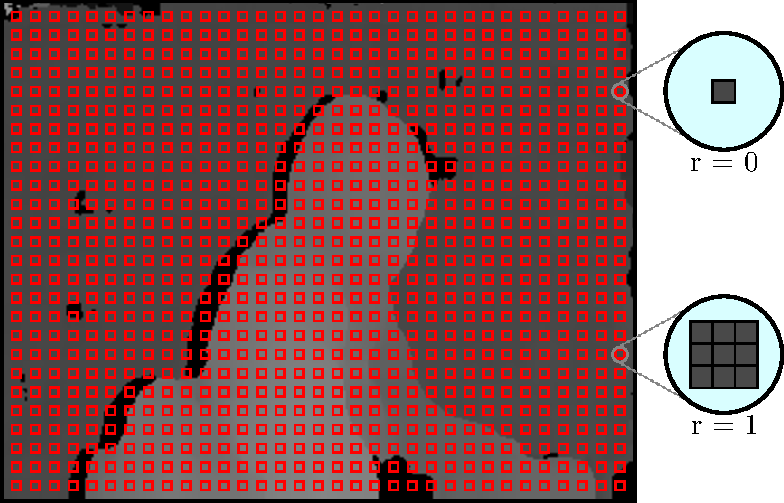
\includegraphics[width=10cm]{img/samplepoints_initmodes.pdf}
	\end{center}
	\caption{Darstellung der Samplepoints mit verschiedenen Radien}
	\label{fig:samplepoints_initmodes}
\end{figure}

\noindent
Nachdem zunächst alle Samplepoints initialisiert wurden, werden die jeweiligen Werte pro Frame aktualisiert. Die eigentliche Erkennung erfolgt dabei einerseits durch die Erstellung einer Pointcloud welche ebenfalls die selben Dimensionen wie die zugrunde liegende Disparity Map besitzt. Erweiternd dazu lässt sich mithilfe der jeweiligen Punkte das als aktuell am gefährlichsten einzustufende Hindernis sowie dessen Position bestimmen. Dabei werden Samplepoints innerhalb der Gefahrenzone zunächst nur auf Bildebene betrachtet.
Zunächst wird die Liste an Samplepoints der errechneten Disparität sortiert.
Da generell Hindernisse direkt vor dem UAV als am kritischsten zu betrachten sind, berechnet der Algorithmus den zweidimensionalen Abstand zwischen Bildhauptpunkt und den Samplepoints mit der geringsten Disparität. 



